\documentclass{article}

\usepackage{verbatim}
\usepackage{amsmath,amsfonts}
\usepackage{enumerate}
\usepackage{fancyvrb}
\usepackage{graphicx}
\usepackage[cm]{fullpage}
\usepackage{float}

\newcommand{\ds}{\ensuremath{\displaystyle}}
\newcommand{\floor}[1]{\ensuremath{\left\lfloor#1\right\rfloor}}
\newcommand{\fracpart}[1]{\ensuremath{\left\{#1\right\}}}

\title{Intermediate Test 4 -- Solutions}
\author{Stellenbosch Camp 2018}
\date{\vspace{-12pt}}


\begin{document}

\maketitle

\begin{enumerate}[1.]

\item % The Phil
\textit{How many numbers from $1$ to $2018$ inclusive can be written as the difference of two perfect squares?}

We say that a number is \emph{nice} if it can be written as the difference of two perfect squares. Any odd number is nice, since $2k+1 = (k+1)^2 -k^2$. Also, any number divisible by $4$ is nice since $4k = (k+1)^2 -(k-1)^2$. So looking at remainders modulo $4$, any number with remainder $0$, $1$ or $3$ is nice; on the other hand, since all perfect squares have remainder $0$ or $1$ modulo 4, the only possibilities for the remainder of a difference of two squares are $0$, $3$ and $1$; hence the numbers with these remainders are precisely the nice numbers.

So to count the nice numbers from $1$ to $2018$, we take the total amount of numbers ($2018$) and subtract those with remainder $2$; since $2018$ has a remainder of $2$ modulo $4$, the amount of the latter is $\floor{\frac{2018}{4}} +1$, yielding a final answer of \[ 2018 - \floor{\frac{2018}{4}} -1 = 1513. \]


\vspace{12pt}
\item %
\textit{Solve for lengths $x$ and $y$ in the following diagram:}

\begin{figure}[h]
\centering
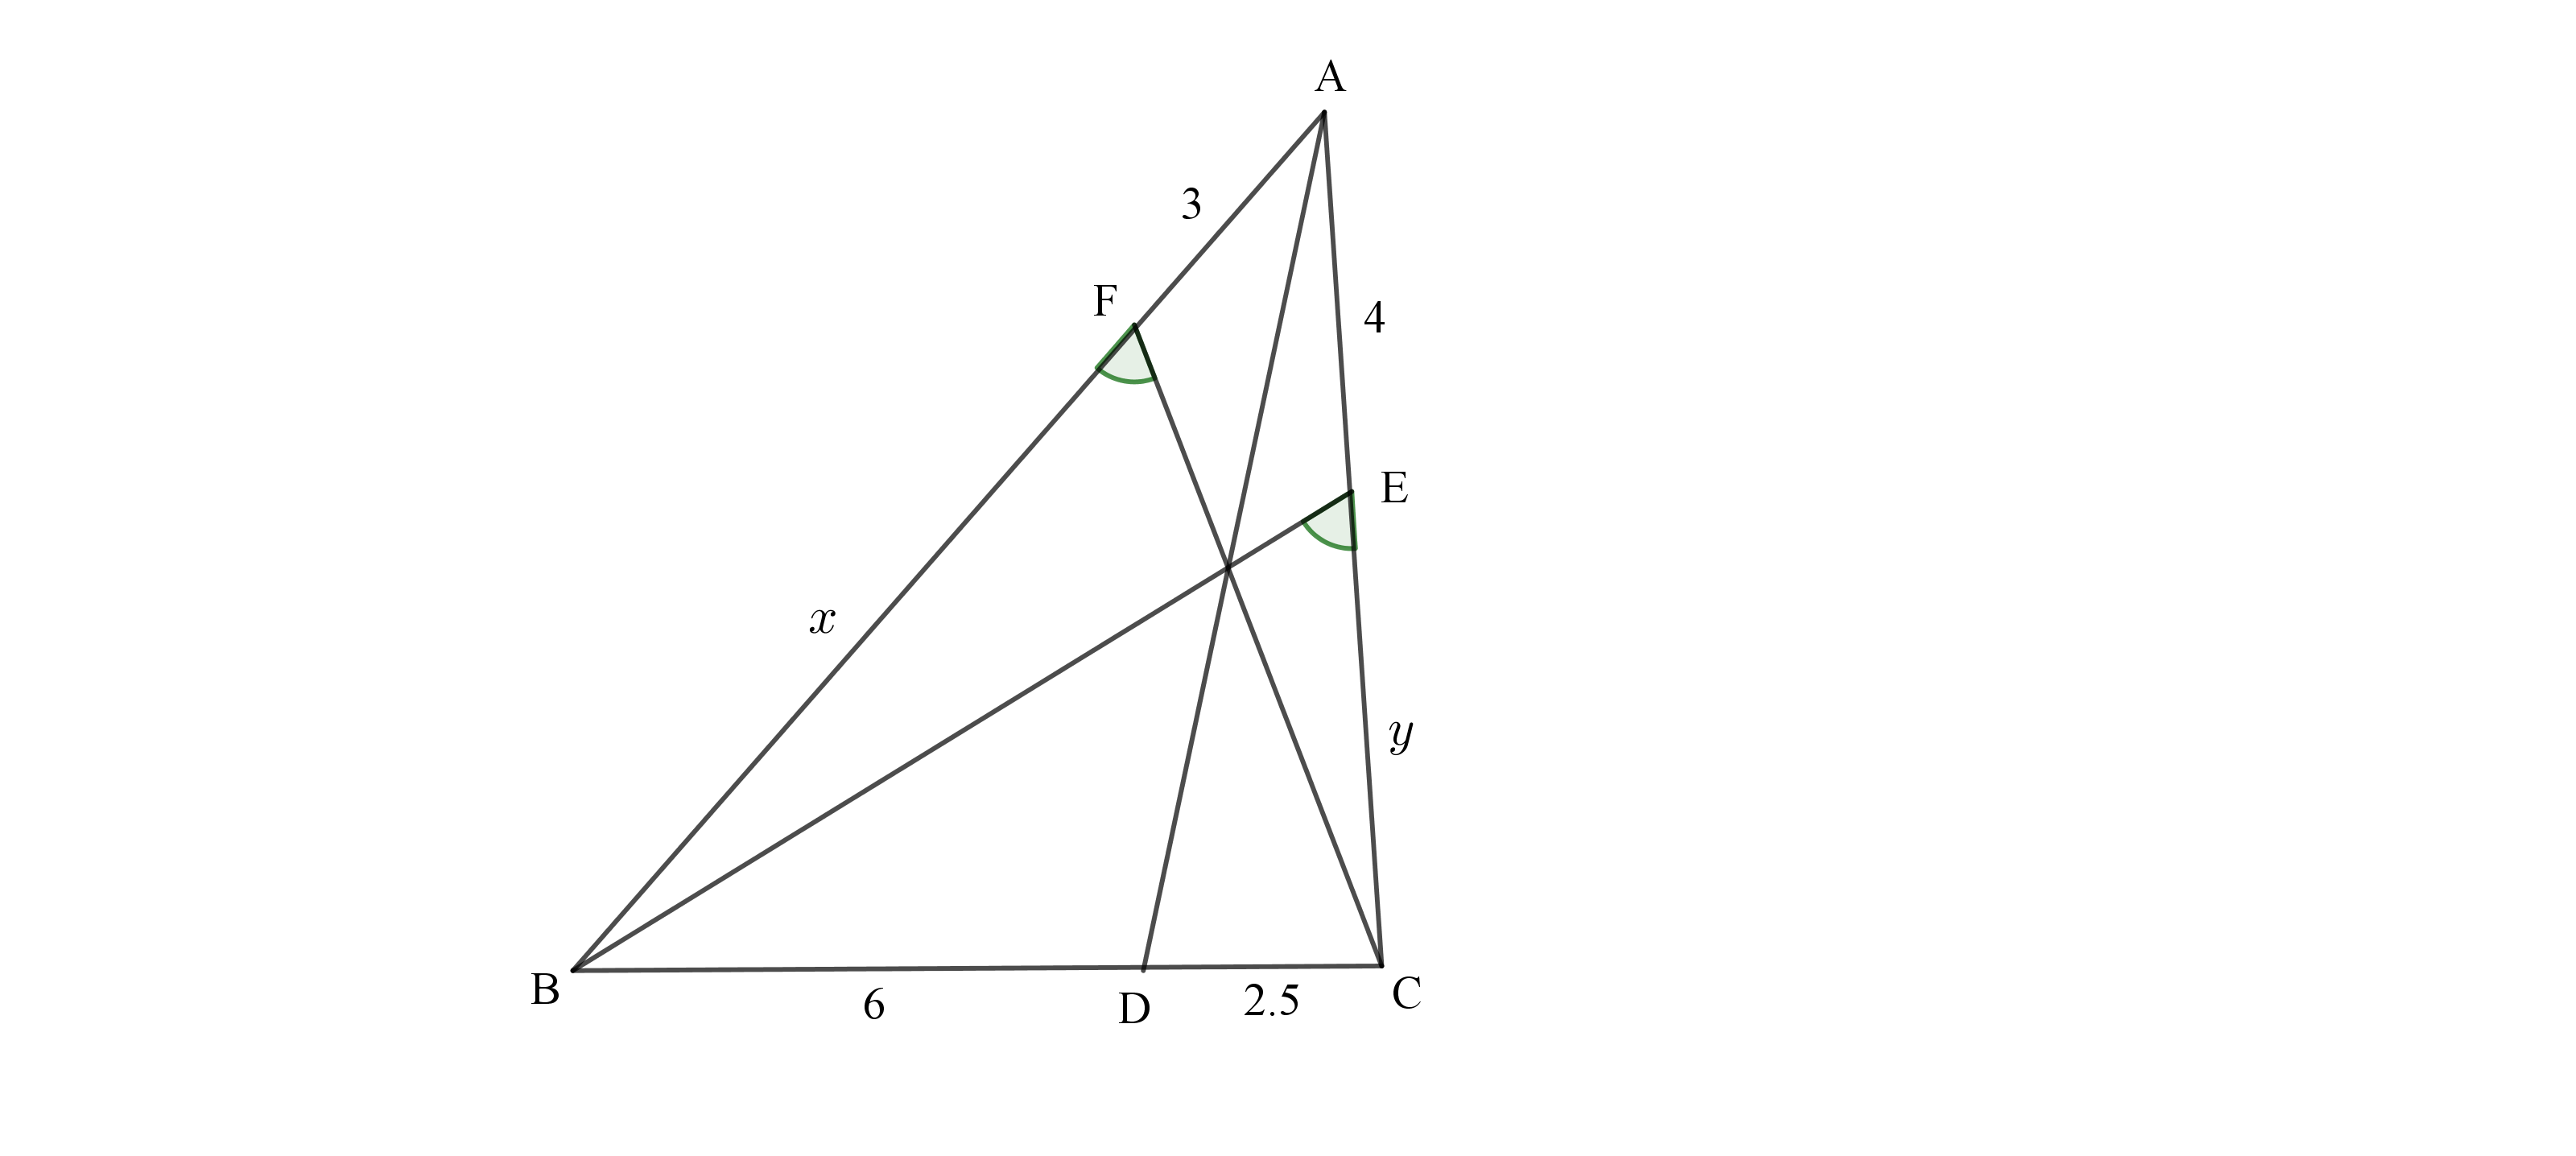
\includegraphics[width=0.6\textwidth]{GeogebraTest4sol.png}
\end{figure}

Label the intersection of the lines through $A$, $B$ and $C$ with sides $BC$, $AC$ and $AB$ as $D$, $E$ and $F$ respectively.
Using Ceva's theorem we have that: 
\begin{equation}
\frac{3}{x} \times \frac{6}{2.5} \times \frac{y}{4} = 1
\end{equation}
Furthermore, since $\angle BFC$ = $\angle BEC$, $BFEC$ is a cyclic quadrilateral. Point A is a point outside the circle passing through $BFCE$, and the lines through $A$ intersects the circle at points $F$, $B$, $E$ and $C$. From Power of a point we know that
\begin{equation}
3(3+x) = 4(4+y)
\end{equation}
Solving equations $(1)$ and $(2)$ simultaneously, we find that $x = 9$ and $y = 5$.


\vspace{6pt}
\item % The Dylan
\textit{Find all functions $f : \mathbb{R} -> \mathbb{R}$ such that for all real numbers $x$, \[ 2 f(x) +3 f(1-x) = x-4x^3. \]}

We take the original equation: $2 f(x) +3 f(1-x) = x-4x^3$. We also take the original equation with $x$ replaced by $1-x$: $2 f(1-x) +3 f(x) = (1-x) -4(1-x)^3 = -3 +11x -12x^2 +4x^3$. Now we multiply the first equation by $2$, the second by $3$, and take the difference between the two, yielding \[ 4 f(x) +6f(1-x) -6 f(1-x) -9 f(x) = 2x -8x^3 +9 -33x +36x^2 -12x^3 = 9 -31x +36x^2 -20x^3. \]
Plugging this back into the original equation, we see that this function satisfies our condition.


\vspace{6pt}
\item % AoPS:  https://artofproblemsolving.com/community/c6t309f6h455752_integers_in_infinite_chessboard
\textit{Prove that it is impossible to write a positive integer in every cell of an infinite chessboard, in such a manner that, for all positive integers $m, n$, the sum of numbers in every $m\times n$ rectangle is divisible by $m + n$.}

Suppose that it is possible. Let $n$ be a positive integer. The sum of the numbers in the $1 \times n$ rectangle with opposite corners at the coordinates $(0, 0)$ and $(n, 1)$ is divisible by $n + 1$. The sum of the numbers in the $1 \times n$ rectangle with opposite corners $(0, 1)$ and $(n, 2)$ is also divisible by $n + 1$. It follows that the sum of the numbers in the $2 \times n$ rectangle with opposite corners at $(0, 0)$ and $(n, 2)$ is divisible by $n + 1$.

However, the sum of the numbers in the $2 \times (n - 1)$ rectangle with opposite corners at $(1, 0)$ and $(n, 2)$ is divisible by $n + 1$, and so we see that the sum of the numbers in the rectangle with opposite corners $(0, 0)$ and $(1, 2)$ is divisible by $n + 1$.

This must be true for every positive integer $n$. It follows that the sum of the numbers in the rectangle with opposite corners $(0, 0)$ and $(1, 2)$ must be $0$. This is a contradiction since we assumed that each square is filled with a positive integer.

\begin{figure}[H]
\centering
\includegraphics[width=0.8\textwidth]{senior_test4_question1_1.mps}
\end{figure}


\vspace{12pt}
\item % Estonia 2007
\textit{An exam with $k$ questions is presented to $n$ students. A student fails the exam if they get less than half the answers right. We say that a question is easy if more than half of the students get it right. Decide if it is possible that}

\vspace{-12pt}
\textit{
\begin{enumerate}
  \item[(a)]  All students fail even though all the questions were easy.
  \item[(b)] No student fails even though no question was easy.
\end{enumerate}
}

\begin{enumerate}
\item[(a)] Consider the total number of correct solutions submitted by all of the students. If all of the students fail, then each student submits strictly fewer that $\frac{k}{2}$ correct solutiona. There are therefore strictly fewer than $\frac{nk}{2}$ correct submissions. On the other hand, if every question is easy, then for each question there are strictly more than $\frac{n}{2}$ correct submissions, and there are thus strictly more than $\frac{nk}{2}$ correct submissions. It is thus not possible for every student to fail if all of the questions are easy.

\item[(b)] We first demonstrate that if either $n$ is odd or $k$ is odd then this is not possible. As before, consider the total number of correct submissions from all of the students. If no students fail then each student solves at least $\frac{k}{2}$ questions and so there are at least $\frac{nk}{2}$ correct submissions in total. Note however that each student solves an integer number of questions, and so if $k$ is odd then this inequality is strict. A similar argument shows that if no question is easy then there are at most $\frac{nk}{2}$ correct submissions, and the inequality is strict if $n$ is odd. Thus if either $n$ or $k$ is odd then these considerations imply that $\frac{nk}{2} > \frac{nk}{2}$, which is a contradiction.

Now suppose that both $n$ and $k$ are even. Let there be $n$ students $S_1, S_2, \dots, S_n$, and $k$ questions $Q_1, Q_2, \dots, Q_k$. Let students $S_1, S_2, \dots, S_{n/2}$ solve questions $Q_1, Q_2, \dots, Q_{k/2}$ and let students $S_{n/2 + 1}, S_{n/2 + 2}, \dots, S_n$ solve $Q_{k/2 + 1}, Q_{k/2 + 2}, \dots, Q_k$. Then each student solves exactly half of the problems and hence no student fails. We also have that every problem is solved by exactly half of the students, and so no question is easy.

\end{enumerate}


\end{enumerate}


\vfill
\centering
\begin{BVerbatim}
 ,    /-.
((___/ __>
/      }
\ .--.(    ___
 \\   \\  /___\
\end{BVerbatim}

\end{document}
